% ------------------------------------------------------------------------------
% SETUP ------------------------------------------------------------------------
% ------------------------------------------------------------------------------

\documentclass[12pt]{article}

\renewcommand{\labelitemi}{$\circ$}
\renewcommand{\labelitemii}{$\circ$}
\renewcommand{\labelitemiii}{$\circ$}

\newcommand{\topo}{\mathcal{T}}
\newcommand{\mani}{\mathcal{M}}
\newcommand{\N}{\mathbb{N}}
\newcommand{\R}{\mathbb{R}}
\newcommand{\RD}{\mathbb{R}^D}
\newcommand{\Rd}{\mathbb{R}^d}
\newcommand{\setN}{\{1, 2, ..., N\}}
\newcommand{\X}{\mathcal{X}}
\newcommand{\x}{\bm{x}}
\newcommand{\Y}{\mathcal{Y}}
\newcommand{\y}{\bm{y}}
\newcommand{\pv}{\bm{p}}
\newcommand{\qv}{\bm{q}}
\newcommand{\W}{\bm{W}}
\newcommand{\M}{\bm{M}}
\newcommand{\Lap}{\bm{L}}
\newcommand{\D}{\bm{D}}
\newcommand{\K}{\bm{K}}
\newcommand{\G}{\bm{G}}
\newcommand{\I}{\bm{I}}
\newcommand{\E}{\bm{E}}
\newcommand{\twonorm}[1]{\left\lVert #1 \right\rVert^2}

\usepackage[a4paper,width = 150mm, top = 25mm, bottom = 25mm, 
bindingoffset = 6mm]{geometry}
\usepackage[utf8]{inputenc}
\usepackage[round, comma]{natbib}
\usepackage{url}
\usepackage[font = footnotesize]{caption}
\usepackage{subcaption}
\usepackage{csquotes} \MakeOuterQuote{"}
\usepackage{ragged2e}
\usepackage{array}
\usepackage{tabularx}
\usepackage[fleqn]{amsmath}
\usepackage{bm}
\usepackage{amssymb}
\usepackage{amsthm }
\usepackage{graphicx}
\usepackage{float}
\usepackage[export]{adjustbox}
\usepackage[table]{xcolor}
% \usepackage{tikz}
%   \usetikzlibrary{trees, arrows, decorations.pathmorphing, backgrounds, 
%   positioning, fit, petri, shapes}
\usepackage{algorithm}
\usepackage{algorithmic}
\usepackage{xcolor, listings}
\usepackage{textcomp}
\usepackage{fancyhdr}
\newcommand{\changefont}{%
    \fontsize{8}{11}\selectfont
}
\usepackage{refcount}
\usepackage[hang,flushmargin]{footmisc} 

\newenvironment{tight_enumerate}{
\begin{enumerate}
  \setlength{\itemsep}{0pt}
  \setlength{\parskip}{0pt}
}{\end{enumerate}}

\DeclareMathOperator*{\argmin}{arg\,min}
\DeclareMathOperator*{\argmax}{arg\,max}

\pagestyle{fancy}
\fancyhead{}
\fancyhead[R]{\changefont{Semi-Supervised Locally Linear Embedding: Application 
and Sensitivity Analysis of Critical Hyperparameters}}
\fancyfoot{}
\fancyfoot[R]{\thepage}
\setlength{\headheight}{14.5pt}
\setlength{\parindent}{0pt}
\interfootnotelinepenalty = 10000

% ------------------------------------------------------------------------------
% MAIN -------------------------------------------------------------------------
% ------------------------------------------------------------------------------

\usepackage{Sweave}
\begin{document}
\Sconcordance{concordance:main.tex:main.Rnw:%
1 92 1 1 0 188 1}


% FRONT PAGE -------------------------------------------------------------------
 
\begin{titlepage}
\begin{center}
    
\LARGE
Seminar Report
    
\vspace{0.5cm}
      
\rule{\textwidth}{1.5pt}
\LARGE 
\textbf{Semi-Supervised Locally Linear Embedding: Application and Sensitivity 
Analysis of Critical Hyperparameters}
\rule{\textwidth}{1.5pt}
   
\vspace{0.5cm}
      
\large
Department of Statistics \\
Ludwig-Maximilians-Universität München
      
\vspace{3.5cm}


\includegraphics[width = 0.4\textwidth]{figures/sigillum.png}

\vspace{3.5cm}

\large
By Lisa Wimmer \\
Under the supervision of Jann Goschenhofer, Ph.D. \\
Munich, April 2\textsuperscript{nd}, 2021

\end{center}
\end{titlepage}

% CONTENTS ---------------------------------------------------------------------

\pagenumbering{Roman}
\newpage

\Large
\noindent
\textbf{Abstract}
\vspace{0.5cm} \\
\noindent
\normalsize
\input{chapters/abstract.Rnw}
\newpage

\Large
\noindent
\textbf{Extended Abstract}
\vspace{0.5cm} \\
\noindent
\normalsize
The goal of this report is to lay out the theoretical framework behind the 
manifold learning technique of \textit{semi-supervised locally linear embedding 
(SS-LLE)}, and to put it to implementation for data sampled from a manifold.

Proposed by \citet{yangetal2006}, SS-LLE extends the local graph-based method 
of \textit{locally linear embedding (LLE)} that had earlier been developed by 
\citet{roweissaul2000} and seen widespread application ever since.

\newpage

\tableofcontents
\newpage

\Large
\noindent
\textbf{List of Symbols}
\vspace{0.5cm} \\
\noindent
\normalsize

\begin{tabularx}{\textwidth}{ 
  >{\raggedleft\arraybackslash}X 
  >{\raggedright\arraybackslash}X}
  $D \in \N$ & Number of observed dimensions \\
  $d \in \N$ & Number of dimensions of embedded manifold \\
  $m \in \N$ & Number of dimensions of low-dimensional representation \\
  $N \in \N$ & Number of observed data points \\
  $\mani \subset \RD$ & $d$-manifold embedded in $\RD$ \\
  $\bm{X} = (\bm{x}_1, \bm{x}_2, ..., \bm{x}_N) \in (\RD)^N$ & Observed 
  coordinates of data sampled from $\mani$ \\
  $\bm{Y} = (\bm{y}_1, \bm{y}_2, ..., \bm{y}_N) \in (\R^m)^N$ & Learned 
  coordinates of low-dimensional representation of data
\end{tabularx}

\newpage

\listoffigures
\newpage
\listoftables
\newpage

% CHAPTERS ---------------------------------------------------------------------

\pagenumbering{arabic}
    
\section{Introduction}
\label{intro}
Machine learning problems increasingly employ data of high dimensionality. 
While a large amount of samples is beneficial to learning, high-dimensional 
feature spaces, such as in speech recognition or gene processing, pose serious 
obstacles to the performance and convergence of most algorithms 
\citep{cayton2005}. 
\\

\textbf{High dimensionality.}
Three aspects strike as particularly problematic: computational operations, 
interpretation of results, and geometric idiosyncrasies.
Computational cost must be considered but is becoming less of an issue with 
technological evolution \citep{leistetal2009}.
By contrast, the demand for explainable results (for reasons of, say, safety or
ethics) is rather intensified by the advance of complex technology. 
Alas, interpretation in more than a few dimensions is virtually inaccessible to 
humans \citep{doshivelezkim2017}. 
The geometric aspect is often addressed as \textit{curse of dimensionality}, a 
term subsuming various phenomena of high-dimensional spaces. 
It is generally not straightforward to infer properties of objects in these 
spaces as geometric intuition developed in lower dimensions can be 
misleading.
Crucially, the exponential increase of spatial volume induces sparsity. 
Consequences of this behavior are, among others, a sharp incline in the number 
of points required to sample the feature space and a loss in meaningfulness of 
distances. 
Many learners, however, rely on these 
concepts\footnote{For instance, consider support vector machines and
$k$-nearest neighbors, both of which rely on distances, or tuning, which often
requires extensive sampling of the hyperparameter space.} and see 
their functionality deteriorate \citep{verleysenfrancois2005}. 
\\

\textbf{Manifold learning.}
These challenges make the case for \textit{dimensionality reduction}, that is, 
the endeavor of compressing problem dimensionality to a manageable size. 
Far from undue simplification, dimensionality reduction is justified by the 
belief that the latent data-generating process is indeed of much lower dimension 
than is observed.
Consider, for example, image data showing objects in different poses.
Such data are typically stored in high-dimensional pixel representations, yet it 
is reasonable to suppose that variation in these images is in fact caused by a 
small number of latent features.
More formally, the data are assumed to lie on a $d$-dimensional 
\textit{manifold} embedded in the $D$-dimensional observation space, with 
$d \ll D$ \citep{cayton2005}.
A crucial property of $d$-manifolds, i.e., the $d$-dimensional generalization of
a curved surface, embedded in $\RD$, is their local topological equivalence to 
$\Rd$ \citep{mafu2011}.
% This locally Euclidean behavior is exemplified by a sphere embedded in $\R^3$: 
% although the sphere as a whole is entirely non-linear, on sufficiently small 
% patches of its surface it behaves just like a flat plane in $\R^2$.
It is precisely this fact that allows manifold coordinates to be mapped to 
$\Rd$ in a reduction of dimensionality\footnote{
The most intuitive example of this is probably the representation 
of the Earth, which is a two-dimensional manifold enclosed in three-dimensional 
space, on two-dimensional maps.}.
The goal is now to learn this mapping in an unsupervised manner 
\citep{cayton2005}.
Mapping manifold coordinates to $\Rd$ is in general not equivalent to simple 
projection onto the $d$-dimensional coordinate hyperplanes.
Instead, models must learn the intrinsic neighborhood structure of the manifold
to establish a notion of "nearness" between points.
Standard distance metrics do not apply (globally) as points on general manifolds 
are connected by curved paths rather than straight lines \citep{mafu2011}.
\\

\textcolor{red}{Adapt to structure of chapter 3}

\textbf{Local graph-based techniques.}
Various approaches have been proposed to retrieve points' manifold coordinates.
A taxonomy may, for example, be found in \citet{vandermaatenetal2009}. 
Many rely on spectral techniques, trying to find a matrix representation of the 
data whose principal eigenvectors are used to span a $d$-dimensional subspace.
% Drawing from the nature of the eigenvalue problem they solve, spectral methods 
% are also referred to as \textit{convex}.
One group of spectral methods attempts to retain global isometry by mapping 
pairwise distances to $\Rd$.
Among them, some are based on Euclidean distances and thus confined to 
learning linear embeddings (such as \textit{principal component analysis (PCA)} 
or \textit{multi-dimensional scaling (MDS)}).
Since linearity is a strong assumption that will not hold for general manifolds, 
non-linear techniques are more widely applicable \citep{vandermaatenetal2009}.
For example, \textit{Isomap} achieves non-linearity by applying geodesic 
distances in the MDS setup \citep{tenenbaumdesilvalangford2000}.
Research indicates, however, that for non-convex manifolds it is more effective 
to preserve local structures only.
Otherwise, solutions are prone to shortcuts, i.e., placing points close in $\RD$
next to each other when they lie in fact on quite different parts of the 
manifold \citep{belkinniyogi2003}.
In order to avoid such miscalculations, sparse techniques focus on merely 
local neighborhood structures, modeled through weighted graph representations.
The information from these graphs is then condensed into a sparse matrix. 
Eventually, the principal eigenvectors of this matrix yield the desired 
low-dimensional coordinates \citep{vandermaatenetal2009}.
\\

\textbf{Locally linear embedding.}
One such local graph-based technique is \textit{locally linear embedding (LLE)}, 
the unsupervised algorithm SS-LLE builds upon \citep{roweissaul2000}.
LLE is based on the idea that the embedded manifold may be approximated by 
locally linear neighborhoods in $\RD$.
Weights for the resulting graph are obtained by linear reconstruction of points 
from their neighbors. 
As these weights are believed to reflect the intrinsic geometry of the manifold, 
they are topological properties and should as such also reconstruct points in 
$d$ dimensions.
LLE thus maps vicinity structures to the $d$-dimensional subspace and finds the 
Euclidean coordinates that preserve them best by means of spectral decomposition \citep{roweissaul2000}.

Much of the theoretical foundation for LLE has been discussed only in later 
work.
In particular, \citet{belkinniyogi2001} proposed \textit{Laplacian eigenmaps}, 
a method which employs the graph Laplacian, and provided evidence for the fact 
that, under certain assumptions, LLE may be generalized to the same framework 
\citep{belkinniyogi2003}.
A later proposition by \citet{donohogrimes2003}, \textit{Hessian LLE (H-LLE)}, 
may be viewed as an algorithmic variant of LLE and a conceptual variant of 
Laplacian eigenmaps (using the Hessian en lieu of the Laplacian).
The theoretical link between LLE and Laplacian eigenmaps, centered around 
the Laplace-Beltrami operator, has recently been found to hold less generally 
than previously assumed \citep{wuwu2018}. 
It still appears beneficial to interpret all methods in this common framework 
also found by \citet{bengioetal2003}; a more thorough study of convergence 
guarantees is left to future research.
\\

\textbf{Semi-supervised extension.}
The above approaches have been shown to successfully retrieve manifold 
structures in different applications \citep{wuwu2018}.
However, their fully unsupervised functionality offers a drawback: they may fail
to find a low-dimensional embedding that has an actual reflection in the 
real-life setting.
Such situations might require the specification of some pre-labeled instances.
Also, it may simply be the case that some observations already come with labels, 
or that annotation of a subset of the data is available at low cost 
\citep{yangetal2006}.
When prior knowledge is at hand it is only natural to use it.
Therefore, \citet{yangetal2006} proposed \textit{semi-supervised locally linear 
embedding (SS-LLE)}, an extension to LLE that is able to harvest prior 
information.
\\

\textbf{Outline.}
Indeed, the presented results indicate considerable success of their technique.
It is the aim of this report to (1) reproduce these results, thereby creating
an open-source implementation of SS-LLE, and (2) to apply SS-LLE to further 
manifold learning tasks for a more thorough assessment of its performance. 
The rest of the report is organized as follows: chapter \ref{math} 
provides a mathematical framework where fundamental concepts are briefly 
introduced; chapter \ref{lgb-mani-learn} explains the framework of local 
graph-based manifold learning; chapter \ref{sslle} presents SS-LLE in detail; 
chapter \ref{experiment} discusses the results of the conducted experiments; and 
chapter \ref{concl} draws final conclusions.









\section{Basic Manifold Theory}
\label{math}
This chapter introduces the main geometric concepts considered necessary to
provide a solid understanding of SS-LLE\footnote{
Obviously, the list of concepts discussed is by no means extensive. Theory is
presented much more in detail (and mathematical rigor) in, for example, 
% FIXME Put in source
\textcolor{red}{good book}.
}.
It must be noted that everything discussed here is presented through the lens of
machine learning, deliberately forsaking the generality inherent to topology.
Therefore, assuming features can be represented by coordinates in 
$D$-dimensional Euclidean space, all concepts are examined with regard to their
meaning in $\RD$.
Dimensionality reduction techniques take the data observed in $\RD$ to actually
lie in a $d$-dimensional topological space that is not necessarily Euclidean but
exhibits some specific properties.
\\

% FIXME Make enumeration more compact 

\textbf{Topological spaces.} A \textit{topological space} is constituted by a 
set $X$ equipped with a \textit{topology} $\topo$. 
A topology is a general way of describing relations between elements in $X$.
Consider a function $\topo: X \rightarrow 2^X, x \mapsto \topo(x)$, which 
assigns to $x \in X$ a set of subsets of $X$ called a \textit{neighborhood}.
For $\topo$ to be a topology\footnote{
Alternative definitions employ open subsets of $X$, see for example 
\citet{waldmann2014}.
}
on $X$, the following properties must hold \citep{brown2006}:
\begin{tight_enumerate}
  \item If $\topo$ is a neighborhood of $x$, then $x \in \topo$.
  \item If $\topo$ is a subset of $X$ containing a neighborhood of $x$, then 
  $\topo$ is a neighborhood of $x$.
  \item The intersection of two neighborhoods of $x$ is again a neighborhood of
  $x$.
  \item Any neighborhood $\topo$ of $x$ contains a neighborhood $\topo^{\prime}$ 
  of $x$ such that $\topo$ is a neighborhood of each element in 
  $\topo^{\prime}$.
\end{tight_enumerate}

Note that, in this general definition, neighborhoods are based on an abstract
notion of "nearness". 
Learning the structure of a topological space effectively boils down to learning 
neighborhood relations.
In Euclidean topological space these are directly based on distance: 
neighborhoods are constructed by $\epsilon$-balls containing all elements within 
a Euclidean distance of $\epsilon$ from $x$. 
The resulting topology is also called the \textit{metric topology} 
\citep{mccleary2006}.

Topological spaces in general are not accessible via distances.
The ultimate goal is again the interpretation of the data in a Euclidean space, 
albeit one with lower dimensionality, where such concepts are meaningful.
The next step is thus to study how a (potentially highly non-linear) topological 
space might relate to $\Rd$.
\\

\textbf{Homeomorphisms.} Consider two topological spaces $(X, \topo_X)$, 
$(Y, \topo_Y)$ (denoted by the respective shorthands $X$, $Y$ from here) and a 
mapping function $f: X \rightarrow Y$. 
If $f$ is bijective and continuous and $f^{-^1}: Y \rightarrow X$ is also 
continuous, $f$ is called a \textit{homeomorphism}.
Intuitively, this is equivalent to $f(\topo)$ being a neighborhood of $f(x)$ if
$\topo$ is a neighborhood of $x$ \citep{brown2006}.
Topological spaces for which such a mapping exists are \textit{homeomorphic} to
each other. 
Any properties of $X$ that $Y$ shares when it is homeomorphic to $X$ are 
referred to as topological properties. 
Two homeomorphic spaces are thus topologically equivalent \citep{mccleary2006}.

If there exists a non-negative integer $d$ such that for every $x$ in a 
topological space $X$ a local neighborhood is homeomorphic to an open subset of 
$\Rd$, $X$ is \textit{locally Euclidean}\footnote{
For locally Euclidean topological spaces it is thus meaningful to speak of
elements as points.
}.
In local neighborhoods $X$ then behaves like $\Rd$, which is conceivably a 
desirable property in the context of manifold learning \citep{mafu2011}.
\\

\textbf{Manifolds.} \textit{Manifolds} are now precisely such locally Euclidean
topological spaces, with some additional properties.
For $\mani$ to be a $d$-dimensional manifold\footnote{
$\mani$ is again a shorthand, omitting the explicit notation of the 
corresponding topology. 
} (also: $d$-manifold) it must meet 
the following conditions \citep{waldmann2014}:

\begin{tight_enumerate}
  \item $\mani$ is Hausdorff.
  \item $\mani$ is second-countable.
  \item $\mani$ is locally homeomorphic to $\Rd$.
\end{tight_enumerate}

The Hausdorff condition is a separation property and ensures that for any two 
distinct points from $\mani$ disjoint neighborhoods can be found 
\citep{brown2006}.
Second-countability restricts the manifold's size via the number of open sets 
it may possess \citep{waldmann2014}.

Manifolds can now be \textit{embedded} in Euclidean space.
Consider $\R^k \supset \Rd$\footnote{
Here, $k$ is used to denote a general higher-dimensional space (a manifold
embedded in $\R^k$ is also embedded in $\R^{k + 1}$, and so on, as 
homeomorphisms are transitive \citep{waldmann2014}). 
This is deliberate to distinguish it from the more specific notation $D$ 
indicating the number of observed features.
}.
$\Rd$ is endowed with the so-called \textit{subspace topology} that results
from intersecting open subsets of $\R^k$ with $\Rd$ (for $\R^2$, these are
$\epsilon$-circles obtained by intersecting $\R^3$-$\epsilon$-balls with the 
coordinate planes).
For a manifold $\mani$, to be embedded in $\R^k$ means that $\mani$ is enclosed
by $\R^k$ but locally homeomorphic to $\Rd$, thereby inheriting the metric
subspace topology from $\Rd$ \citep{waldmann2014}.
It can be shown that $k = 2d + 1$ is sufficient to create an embedding, but $k$
may be smaller \citep{mafu2011}.

This now has important consequences for manifold learning: data lying on a 
$d$-dimensional manifold $\mani$ embedded in $\RD$ are observed as 
$D$-dimensional points but may locally be treated like points from $\Rd$.
\\

\begin{minipage}[b]{0.5\textwidth}
  Figure \ref{fig:scurve} shows the well-known \textit{S-curve} manifold embedded 
  in $\R^3$.
  Clearly, the S-curve as a whole is far from linear, but local patches on its
  surface behave like planes from $\R^2$.
  So the S-curve is two-dimensional and feature dimensionality can in effect be 
  compressed from $\R^3$ to $\R^2$.
  The challenge is now to unravel the manifold in a way that preserves its 
  structure to maximum extent.
  Obviously, a simple projection to $\R^2$ will not accomplish this task.
  Instead, manifold learning must capture the intrinsic neighborhood structures
  and map these to $\R^2$, which, in this case, can be imagined as a 
  "flattening-out" of the S-curve.
\end{minipage}
\begin{minipage}[b]{0.1\textwidth}
  \phantom{space}
\end{minipage}
\begin{minipage}[b]{0.4\textwidth}
  \begin{figure}[H]
    \centering
    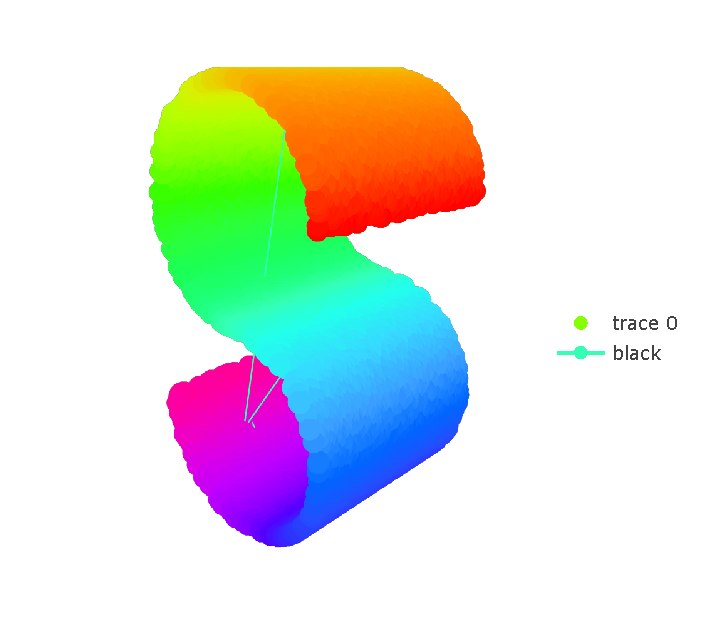
\includegraphics[trim = 100 20 100 20, clip, 
      width = \textwidth]{figures/s-curve}
    \caption[S-curve manifold]{10,000 points sampled from the S-curve manifold 
    as implemented in \texttt{Python}'s \texttt{scikit-learn} library 
    \citep{scikit-learn}.}
    \label{fig:scurve}
  \end{figure}
\end{minipage}

\vspace{0.5cm}

\textbf{Geodesics.} One last aspect remains open, namely how to handle distances 
on manifolds.
Figure \ref{fig:scurve} illustrates that standard Euclidean distances are not
meaningful here: rather than measuring "shortcuts" between points across 
$\R^3$ (where, for instance, points in the red upper area would be considered
quite close to points in the cyan mid area), it makes intuitive sense to 
constrain distances to the manifold surface.
In order to enable the construction of such a metric, manifolds must fulfill
two additional properties: being \textit{Riemannian} and being 
\textit{connected} \citep{mafu2011}.
The Riemannian property is based on differentiability and ensures that concepts 
of curvature, length and angle remain meaningful \citep{mafu2011}.\footnote{
A detailed derivation is beyond the scope of this report and may be found, for
example, in \citet{mukherjee2015}.
}
Connectedness means that no separation $\{ U, V\}$ of a manifold $\mani$
exists with open, non-empty and disjoint $U, V \subset \mani$, 
$\mani = U \cup V$.
For manifolds, connectedness is immediately equivalent to path-connectedness.
Informally stated, any two points on a connected manifold can be linked by a 
path
% Such a path is a continuous function $\lambda: [0, 1] \rightarrow \mani$ with
% $\lambda(x) = 0$ and $\lambda(y) = 1$ for any two points $x, y \in \mani$
\citep{mccleary2006}.

For connected Riemannian manifolds it is now possible to define a distance 
metric, or \textit{geodesic distance}.
Geodesic distance is the length of the shortest curve (\textit{geodesic}) on
$\mani$ between two points on $\mani$, as measured by arc-length\footnote{
Geodesics are but a peripheral note here; for a precise definition see for 
example \citet{mafu2011}.
} (such 
a curve must exist due to connectedness).
Intuitively, geodesic distance can be identified with Euclidean distance in
Euclidean spaces where shortest curves are but straight lines \citep{mafu2011}.

% A curve $c$ in $\mani$ is a smooth mapping from an open interval 
% $\Lambda \subset \R$ into $\mani$. 
% $c$ is parametrized by a point $\lambda \in \Lambda$, such that 
% $c(\lambda) = (c_1(\lambda), ..., c_d(\lambda))^T$ (all $c_j, j = 1, ..., d$,
% having a sufficient number of continuous derivatives) is a curve in $\Rd$.
% Component-wise differentiation with respect to $\lambda$ yields the 
% \textit{velocity} of $c$ in $\lambda$, $c^{\prime}(\lambda) =
% (c_1^{\prime}(\lambda), ..., c_d^{\prime}(\lambda))^T$.
% The \textit{speed} of $c$ is given by $\| c^{\prime}(\lambda) \|^2_2$, where
% $\| \cdot \|^2_2$ denotes the square norm.
% Then, distance along this curve is measured by the arc-length 
% $L(c) = \int_{\pv}^{\qv} \| c^{\prime}(\lambda) \|^2_2 d\lambda$.
% 
% Finally, geodesic distance can be derived as the length of the shortest such
% curve, out of the set of differentiable curves in $\mani$ that connect $\pv$ and 
% $\qv$, $\mathcal{C}(\pv, \qv)$: \\
% $d^{\mani}(\pv, \qv) = \inf_{c \in \mathcal{C}(\pv, \qv)} L(c)$ 
% \citep{mafu2011}. 





\section{Local Graph-Based Manifold Learning (LGML)}
\label{lgb-mani-learn}
\subsection{Overview and Conceptual Framework}
\label{principles-overview}

After the goal of manifold learning has been formalized, it shall now be laid 
out how the problem is approached by LLE as the conceptual parent of SSLLE 
(the incorporation of prior information is a rather different matter that will 
be addressed in chapter \ref{sslle}). 
Much of the theoretical foundation for LLE has been discussed only in later 
work.
In order to provide a more integrated background, explanations will therefore be 
given in a broader context of local graph-based manifold learning, which also 
comprises LEM and HLLE.
The particular relationship of the three methods shall be made clear along the 
way.

Local graph-based manifold learning arises from a variety of geometric 
intuitions and computational implementations.
Nonetheless, methods share common structures that allow for interpretation in a 
more abstract framework (\citet{bengioetal2003}, \citet{bengioetal2004}).
It should be noted that such a framework might be established from several 
angles; after all, the different methods attempt to solve the same problem 
and can thus often be translated into one another.

Figure \ref{fig:models-overview} depicts a schematic overview on the models 
studied here, representing the specific perspective taken within this report.
All of these belong to the realm of \textit{spectral} models.
The non-spectral group includes, for instance, techniques based on neural 
networks and is not discussed here \citep{vandermaatenetal2009}.

\begin{figure}[H]
    \centering
    % https://docs.google.com/drawings/d/1982RyrkrJzhR-LHvR3xUmuCMEdpiK8qkm00HBvKMY9I/edit
    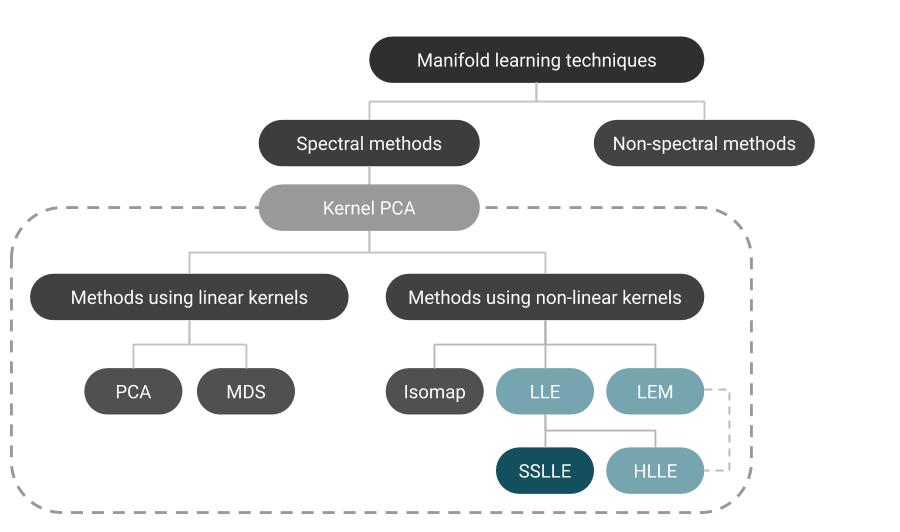
\includegraphics[trim = 0 0 0 0, clip, % left bottom right top
      width = \textwidth]{figures/models-overview}
    \caption[Overview on selected manifold learning models]{A schematic overview 
    on selected methods of manifold learning (the list is by no means extensive 
    and could arguably be ordered in several alternative ways). 
    \textit{Source:} own representation, inspired by a similar example given in 
    \citet{vandermaatenetal2009} and re-interpreted with the findings in 
    \citet{bengioetal2004}.}
    \label{fig:models-overview}
  \end{figure}

As visually indicated in figure \ref{fig:models-overview} , this report will 
sketch the idea behind local graph-based manifold learning in the light of 
\textit{kernel principal component analysis (kernel PCA)}.
Kernel PCA was actually proposed first and later shown to link the other 
concepts by a unified idea (\citet{hametal2003},
It makes for an appealing framework that, firstly, provides a useful general 
intuition to manifold learning, and, secondly, subsumes the other methods in a 
way that proves beneficial for the important task of out-of-sample extension \citep{bengioetal2004}.
\\

\textbf{Kernel PCA.} Kernel PCA builds upon two fundamental concepts 
in machine learning: it performs \textit{principal component analysis (PCA)} on 
data transformed by the \textit{kernel trick}.
In principle, it undertakes two subsequent steps.
First, features of interest are extracted from the data by kernelization. 
These are taken to capture the intrinsic data structure and may therefore be 
understood as an approximation to the latent manifold properties.
In the end, they constitute a matrix representation.
Second, \textit{principal component analyis (PCA)} finds the principal axes 
along which these intrinsic properties vary, yielding the desired reduction in 
dimensionality by preserving the most relevant latent dimensions \citep{schoelkopfetal1998}.

\begin{itemize}

  \item[] \textbf{Kernelization.} By kernelization, i.e., mapping the data to a 
  space $\mathcal{F}$ of arbitrarily high dimension, features may be obtained 
  that relate to the input in a possibly non-trivial way\footnote{
  Support vector machines use the kernel trick to achieve linear separability. 
  An intuitive example may be given by data observed in two classes that form 
  concentric circles in $\R^2$. 
  While such data are not linearly separable in two dimensions, they are in three: 
  mapping the classes to different heights enables separation by a horizontal 
  hyperplane.
  This example also hints at the idea of (spectral) clustering to which kernel 
  PCA is indeed intimately related \citep{bengioetal2004}.
  }.
  Crucially, the feature map $\phi: \RD \rightarrow \mathcal{F}$ need not be 
  computed explicitly (this might prove prohibitively expensive).
  Kernelization instead solely relies on inner products $\langle \phi(\x_i), 
  \phi(\x_j) \rangle$ of the transformed inputs.
  Employing Mercer's theorem of functional analysis, these inner products may 
  be interpreted as performed by a continuous kernel 
  % Remove domain and co-domain of kappa, might be wrong, needs the Hilbert 
  % space after all, right
  $\kappa(\x_i, \x_j)$ in some space with Hilbert property.
  Appropriate choice of $\kappa$ then allows for the data to be represented by a 
  matrix $K \in \R^{N \times N}, K_{ij} = \kappa(\x_i, \x_j)$.
  This matrix is the numerical data representation derived with respect to their 
  latent properties. \citep{schoelkopfetal1998}.
  Precisely how it is computed depends on the choice of the kernel function 
  $\kappa$ and gives rise to different techniques \citep{hametal2003}.
  
  \item[] \textbf{PCA.} PCA is a quite powerful technique by itself.
  It finds the directions of maximum variance through eigenanalysis of the 
  empirical covariance matrix, yielding the most important axes of inter-feature 
  relations that coincide with the principal eigenvectors of the covariance 
  matrix (for comments on eigenanalysis see chapter \ref{eigenanalysis} of the 
  appendix).
  The data are projected into the linear subspace spanned by these $d$ 
  eigenvectors, thereby mapping the observations to a coordinate system given 
  by those linear feature combinations that represent the strongest 
  (co)variability.
  PCA thus performs an orthogonal input transformation that allows for 
  dimensionality reduction at minimal information loss \citep{cayton2005}.
  In kernel PCA, this eigenanalysis is implicitly performed in the feature space 
  $\mathcal{F}$.
  Algorithmically, it boils down to diagonalizing the kernel matrix $K$ 
  \citep{schoelkopfetal1998}.
 
\end{itemize}

Figure \ref{fig:spirals} attempts to visualize the idea of kernel PCA.
The original data (\textit{left}) are observed in two dimensions but clearly 
intrinsically one-dimensional, where the latent manifold feature is expressed by 
coloring. 
The kernel trick creates a non-linear map, visualized here as a projection of 
the intrinsic feature to a third coordinate axis (\textit{middle}). 
Coercing the data to this dimension as the sole axis of variation yields the 
desired one-dimensional representation (\textit{right}). 

\begin{figure}[H]
  \centering
  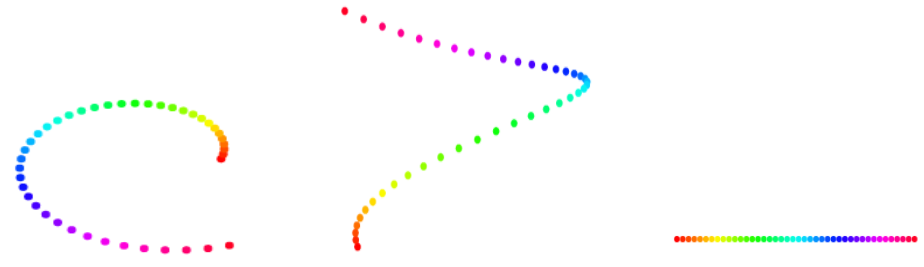
\includegraphics[width = \textwidth]{figures/spirals}
  \caption[Schematic idea of kernel PCA]{Schematic idea of kernel PCA: from data
  observed in two dimensions, but clearly of intrinsic dimensionality one 
  (\textit{left}), create a mapping to a higher-dimensional feature space 
  (\textit{middle}), reduction of which to its principal axes yields the desired 
  one-dimensional representation (\textit{right}).
  \textit{Source:} own representation, using a subset of \texttt{mlbench}'s 
  noise-free \texttt{spirals} data. Note that this is but a schematic depiction 
  where the mid and right representation have not been created by an actual 
  implementation of kernel PCA.}
  \label{fig:spirals}
\end{figure}

% ------------------------------------------------------------------------------

\subsection{Aspects of Local Graph-Based Techniques}
\label{lgb-properties}

% ------------------------------------------------------------------------------

\subsubsection{Non-Linearity and Locality}
\label{nonlin-local}

If kernel PCA sounds like a powerful concept, the crux of course lies in 
finding an appropriate kernel function.
The nature of the feature map applied to the input data determines the kind of 
mapping that may be learned and serves to distinguish the various techniques.
As foreshadowed in figure \ref{fig:models-overview}, spectral methods decompose 
into groups using \textit{linear} and \textit{non-linear} kernels, respectively.
This distinction now directly translates to the feature map $\phi$.
Linear methods suffer from the confinement to finding linear subspaces \citep{vandermaatenetal2009}.
PCA in its standard form can be interpreted as kernel PCA by identifying the 
kernel function with the covariance function.
It thus returns the subspace of greatest variability in the original input 
features \citep{hametal2003}.
The closely related \textit{multi-dimensional scaling (MDS)} approach yields the 
same result, albeit from a different intuition \citep{sauletal2006}.
\\

\textbf{Non-linearity.} As extensively discussed above, $\X$ must often be 
assumed to lie on a non-linear manifold $\mani \subset \RD$, which is precisely 
why kernelization is usually performed such that the resulting feature space is 
related to the input space in a non-linear way \citep{schoelkopfetal1998}.
Conceivably, there is no obvious way to arrive at such a mapping.
\textit{Graph-based} models therefore approach the problem from an alternative 
angle.
In fact, they do not even perform kernelization explicitly: they transform the 
data in a way that can be shown to correspond to applying a (data-dependent) 
kernel function\footnote{
The report does not discuss the actual kernel function as their illustrative 
ability is rather limited.
For an explicit formulation of kernels in LLE, LEM and HLLE see for example \citet{bengioetal2004} and \citet{weinbergeretal2004}.
}, 
but the fundamental intuition is a different one. 
The key idea in graph-based learning is to approximate the manifold by a 
discretized graph representation.
Such a graph may be intuitively imagined as a skeletal model 
of the manifold surface.
The graph properties -- essentially an approximation of the latent manifold 
properties -- are described by functionals that vary across methods.
Eigenanalysis of the associated matrix representation then leads to the 
sought-for low-dimensional subspace coordinates \citep{sauletal2006}.
\\

\textbf{Locality.} The second desideratum in general manifold learning is the 
ability to treat highly non-linear manifolds with sufficiently local focus.
Non-convexity means $\mani$ is isometric to a non-convex subset of Euclidean 
space \citep{donohogrimes2003}. 
Intuitively, such behavior requires careful tracing of the manifold surface.
Local graph-based methods therefore focus on solely local manifold properties, 
and, in doing so, produce sparse matrix representations \citep{cayton2005}.
They are frequently contrasted to \textit{Isomap}, one of the 
earliest and most prominent examples of global manifold learning.
Isomap retains pairwise distances between points on the manifold surface as 
measured along graph edges via geodesic curves\footnote{
It is thus a non-linear variant of MDS, which uses standard Euclidean distances 
\citep{tenenbaumdesilvalangford2000}.
} \citep{tenenbaumdesilvalangford2000}.
Its central assumptions are global isometry and convexity of the parameter 
space \citep{tenenbaumdesilvalangford2000}.
While it yields good results in many applications, Isomap does not sufficiently 
account for the curvature of strongly non-convex manifolds.
In order to avoid this drawback, local methods limit isometry to only hold 
between neighboring points and relax the parameter space 
condition to open, connected subspaces \citep{donohogrimes2003}.

% ------------------------------------------------------------------------------

\subsubsection{Neighborhood Graphs}
\label{algo-common}

Besides the common theoretical framework, LLE, LEM and HLLE also share a general 
algorithmic structure.
It might be summarized as follows \citep{bengioetal2003}:

\begin{tight_enumerate}
  \item Construct a neighborhood graph $\mathcal{G}$ from the observed data.
  \item Analyze the graph properties with an appropriate functional and derive 
  a matrix representation $M$ thereof.
  \item Find the eigenvalues and associated eigenvectors of $M$.
  \item From the principal (top or bottom) eigenvectors, as determined by the 
  ordered eigenvalues, retrieve the low-dimensional coordinates.
\end{tight_enumerate}

\textbf{Neighborhoods.} All local graph-based methods fundamentally 
build on neighborhood graph approximations of the manifold surface.
A neighborhood of $\x \in \X$ is a subset of $\X$ containing another, open 
subset of $\X$ of which $\x$ is an element.
Members of the neighborhood are called neighbors of $\x$.
In metric spaces neighborhoods are defined via distances and therefore 
translate to open balls around each point \citep{waldmann2014}.
This distance-based construction locally applies to manifolds as a direct 
consequence of their local isometry to the Euclidean observation space 
\citep{mafu2011}.
There are two principal ways to build a neighborhood around $\x \in \X$, 
both of which usually employ the squared Euclidean norm\footnote{
In principle, alternative metrics are equally applicable, for instance such 
that measure angles \citep{belkinniyogi2004}.
} $\| \cdot \|^2$.
Let $\mathcal{N}: \X \rightarrow \X^{\ell}, \x \mapsto \mathcal{N} (\x)$ be a 
constructor that assigns a set of neighbors to $\x$.
The first possibility is to restrict the size of the neighborhood to the $k$ 
points with the smallest distance to $\x$, such that
$\ell = k$ and $\mathcal{N}_k(\x) = \{\x_j \in \X: 
\| \x - \x_j \|^2 \leq \gamma\}$, with $\gamma \in \R$ being the $k$-th instance 
of ordered pairwise distances.
Alternatively, the neighborhood may be constructed by collecting all points that
have a maximum distance of $\epsilon \in \R$ to $\x$, yielding 
$\mathcal{N}_{\epsilon} (\x) = 
\{\x_j \in \X: \| \x - \x_j \|^2 \leq \epsilon\}$ and 
$\ell = |\mathcal{N}_{\epsilon} (\x)|$ \citep{heetal2005}.
Both $k$ and $\epsilon$ are hyperparameters that must be specified up-front.
Their choice reflects beliefs about the topological structure of $\mani$ -- 
smaller neighborhoods corresponding to a higher degree of non-linearity -- and 
may affect performance rather strongly \citep{sudderth2002}.
\\

\textbf{Neighborhood graphs.}
$\mani$ can now be characterized by a \textit{neighborhood 
graph} $\mathcal{G} = (\mathcal{V}, \mathcal{E})$, still assuming it is 
sampled well by $\X$. 
Inputs $\x \in \X$ form vertices $\mathcal{V}$ and edges $\mathcal{E}$ 
indicate neighborhood relations \citep{belkinniyogi2001}.

\begin{minipage}[b]{0.5\textwidth}
  Each vertex is connected to its $k$ nearest neighbors or all points 
  within $\epsilon$-radius, depending on the neighborhood definition.
  It is easy to see that $k$-neighborhoods are an asymmetric notion; for one 
  point to be among another's $k$ nearest neighbors the reverse need not be 
  true.
  $k$-neighborhoods therefore lead to directed graphs.
  Conversely, the $\epsilon$-distance boundary holds in both directions and 
  produces undirected graphs \citep{heetal2005}.
  % A fictional example for a directed graph is given by figure 
  % \ref{fig:neighbor-graph}, showing $k$-neighborhoods for seven data points 
  % ($k = 2$).
  Figure \ref{fig:neighbor-graph} shows how a neighborhood graph may be used as 
  an approximation for the example of the S-curve manifold.
  It was built using $k$-neighborhoods with $k = 3$.
  Note that no information on the latent manifold coordinates is required.
\end{minipage}
\begin{minipage}[b]{0.05\textwidth}
  \phantom{xxx}
\end{minipage}
\begin{minipage}[b]{0.45\textwidth}
  \begin{figure}[H]
    \centering
    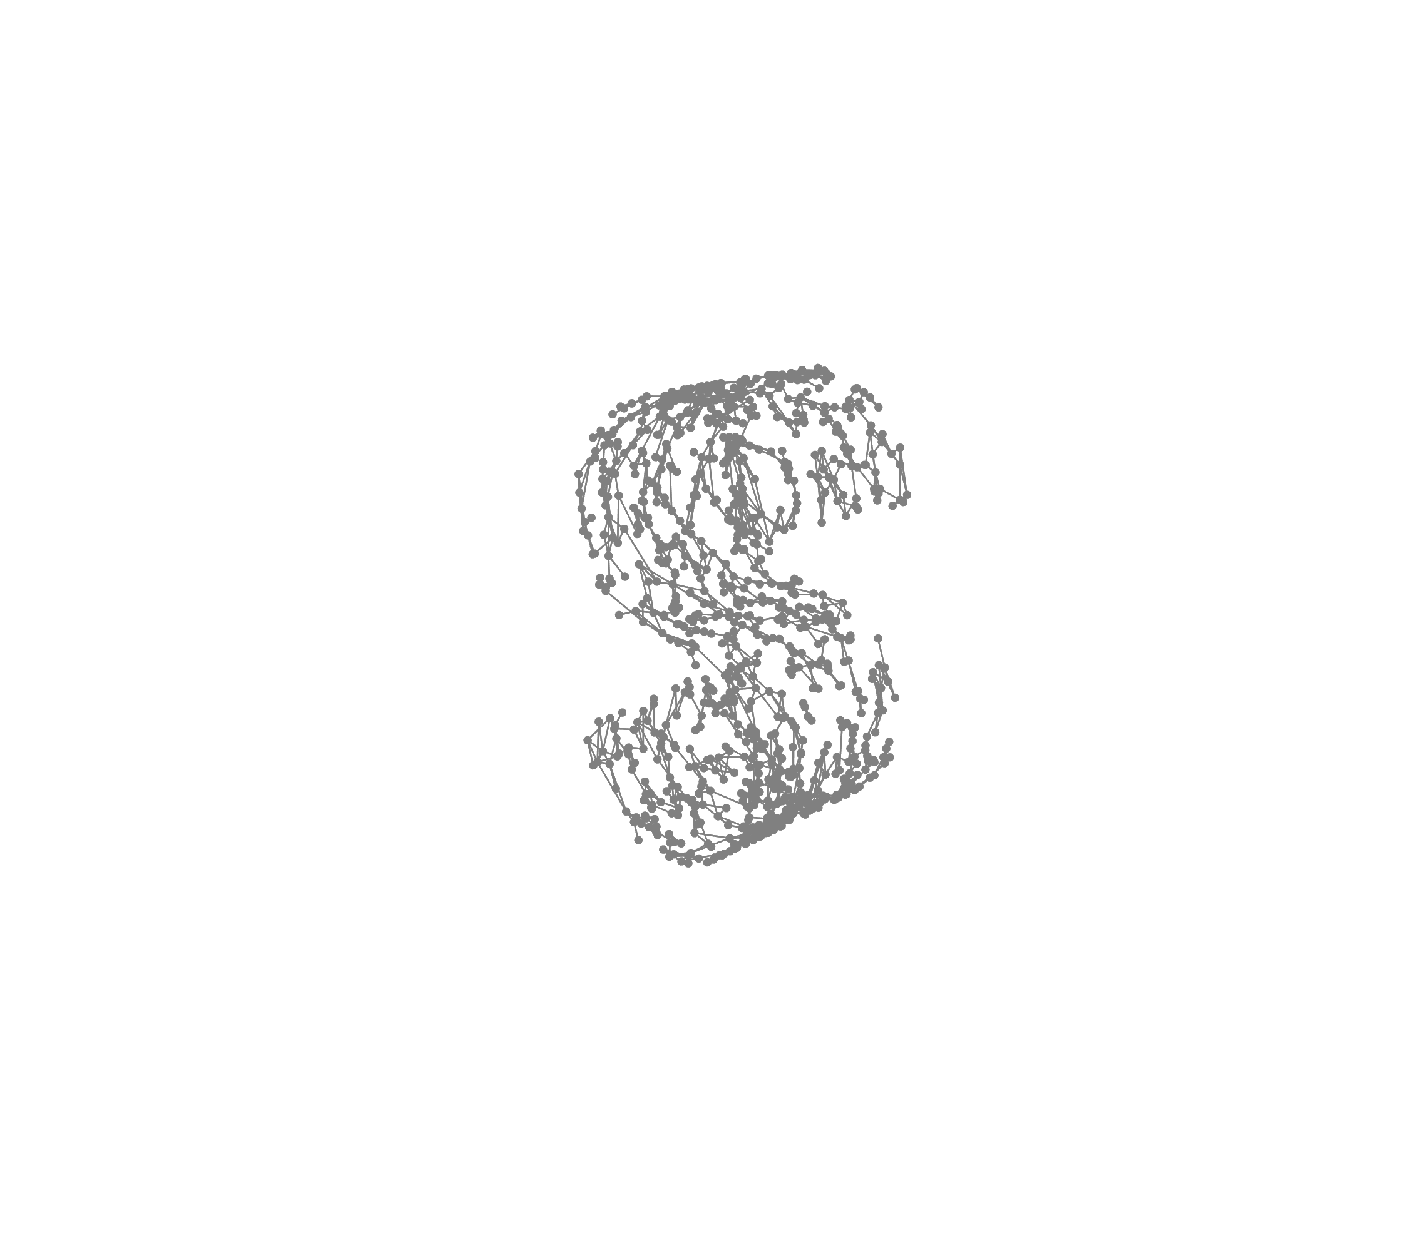
\includegraphics[trim = 250 170 200 100, clip, % left bottom right top
      width = 0.8\textwidth]{figures/s-curve-connected}
    \caption[S-curve neighborhood graph]{$k$-neighborhood graph for 300 points 
    sampled from the S-curve with $k = 5$.
    \textit{Source:} own representation.}
    \label{fig:neighbor-graph}
  \end{figure}
\end{minipage}

% ------------------------------------------------------------------------------

\subsection{Unsupervised Techniques}
\label{techniques}

% ------------------------------------------------------------------------------

\subsubsection{Laplacian Eigenmaps (LEM)}
\label{laplace}

\begin{itemize}
  \item Notion of locality
  \item Laplacian eigenmaps
\end{itemize}

% ------------------------------------------------------------------------------

\subsubsection{Locally Linear Embedding (LLE)}
\label{lle}

\begin{itemize}
  \item Notion of local linearity
  \item Approximation of graph Laplacian
\end{itemize}

% TODO Regularized version???

% ------------------------------------------------------------------------------

\subsubsection{Hessian Locally Linear Embedding (HLLE)}
\label{hlle}

\begin{itemize}
  \item Hessian instead of Laplacian (eigenmaps)
  \item Hessian instead of LS fit (LLE)
\end{itemize}


\section{LGML Techniques}
\label{techniques}
\subsection{Unsupervised Techniques}
\label{unsupervised}

% ------------------------------------------------------------------------------

\subsubsection{Laplacian Eigenmaps (LEM)}
\label{laplace}

The reason for LEM to appear in this report alongside the LLE family is its 
underlying theory both providing a foundation for LLE \citep{belkinniyogi2003}, 
which was originally proposed lacking such, and closely relating to the 
theoretical concepts in HLLE \citep{donohogrimes2003}.

LEM are centered around the preservation of locality, i.e., mapping nearby 
inputs to nearby outputs.
Locality is enforced via the \textit{Laplace-Beltrami operator} defined on 
smooth, compact manifolds, and operationalized by means of the \textit{graph Laplacian} acting as a discrete approximator \citep{belkinniyogi2003}.
This idea is best understood recalling that the similarity of outputs for 
similar inputs is essentially a notion of smoothness and can thus be controlled 
by a size constraint on the gradient of the mapping function.
\\

\textbf{Laplace-Beltrami operator.}
Consider the twice differentiable function $f: \mani \rightarrow \R$ mapping 
two points $\pv, \qv \in \mani$ to $f(\pv)$ and $f(\qv)$, respectively. 
On $\mani$ they are connected by a length-parametrized curve $c(t)$.
Denote the geodesic distance between $\pv$ and $\qv$ by $\ell$, such that
$\pv = c(0)$ and $\qv = c(\ell)$.

\begin{minipage}[b]{0.65\textwidth}
  Gradients of $f$ with respect to $\pv$ are defined in the local tangent space
  $T_{\pv}(\mani)$ spanned by vectors tangent to $\mani$ at $\pv$.
  As $\mani$ is embedded in $\RD$, its tangent spaces are Euclidean and of 
  dimension $d$, i.e., $d$-dimensional hyperplanes \citep{sudderth2002} as 
  depicted in figure \ref{fig:sphere-tangent}.
  If $\pv$ is identified with the origin of $T_{\pv}(\mani)$, the tangent space
  inherits an orthonormal coordinate system obtained from endowing
  $T_{\pv}(\mani)$ with the inner product from $\Rd$ \citep{donohogrimes2003}.
  With this, the distance $|f(\pv) - f(\qv)|$ of mappings can be expressed as
  the length of the integral
  $\int_0^{\ell} \langle \nabla f(c(t)), c^{\prime}(t) \rangle dt$.
  In other words, the geodesic curve connecting $\pv$ and $\qv$ is projected 
  onto $T_{\pv}(\mani)$, and the length of this projection depends on the 
  gradient of $f$ and the curve velocity.
\end{minipage}
\begin{minipage}[b]{0.05\textwidth}
  \phantom{xxx}
\end{minipage}
\begin{minipage}[b]{0.3\textwidth}
  \begin{figure}[H]
    \centering
    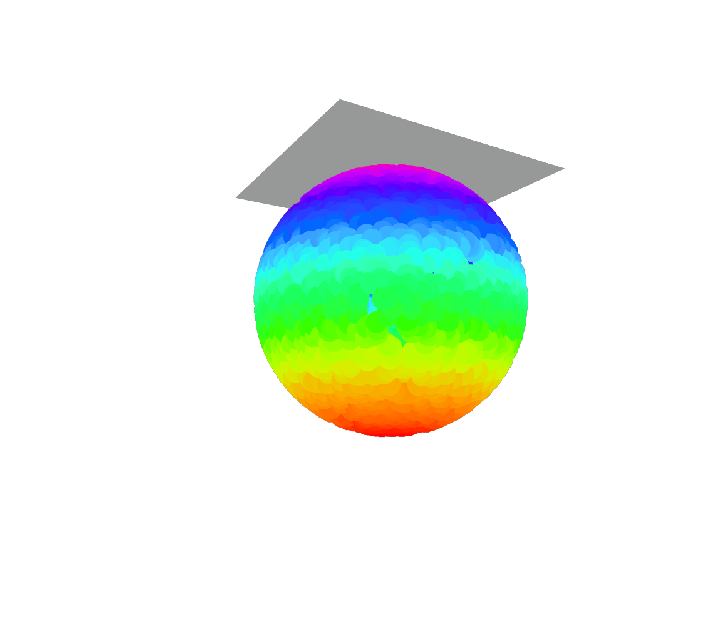
\includegraphics[trim = 90 70 60 30, clip, % left bottom right top
      width = 0.8\textwidth]{figures/sphere-tangent}
    \caption[Tangent hyperplane for two-dimensional unit sphere]{Tangent 
    hyperplane for an exemplary point on the two-dimensional unit sphere 
    manifold, embedded in $\R^3$. \textit{Source:} own representation.}
    \label{fig:sphere-tangent}
  \end{figure}
\end{minipage}

Exploiting the Schwartz equality and relations proved in 
\citet{belkinniyogi2008}, it
can be shown that 
$|f(\pv) - f(\qv)| \leq \| \nabla f(\pv) \| \cdot \| \pv - \qv\| + o$, where 
$o$ marks a term of vanishing size. 
Acknowledging the fact that the distance between $\pv$ and $\qv$ is a datum,
$\| \nabla f \|$ controls how far apart points are mapped on the real line.
Consequently, the goal is to find a mapping that, on average, preserves 
locality, by posing a second-order penalty on $\| \nabla f \|$ and minimizing $\int_{\mani}\| \nabla f \|^2$.
This is just equal to minimizing $\int_{\mani} \mathcal{L}(f)f$ with the 
Laplace-Beltrami operator $\mathcal{L}$ \citep{belkinniyogi2003}.
Applying the operator $\mathcal{L}$ to $f$ again results in a function from the 
same function space as $f$, and for $\mathcal{L} f = \lambda f$, $f$ is an 
eigenfunction of $\mathcal{L}$ with $\lambda \in \R$ as its associated 
eigenvalue.
Crucially, these eigenfunctions are orthogonal for $\mathcal{L}$ and their  
eigenvalues are real, meaning they are natural candidates for forming a 
functional basis \citep{levy2006}.
The optimal embedding map is then given by the $d$ principal eigenfunctions of
$\mathcal{L}$ after removing the bottom one which would map $\mani$ to a 
single point \citep{belkinniyogi2003}.
\\

\textbf{Graph Laplacian.}
Now the same reasoning can be applied to the neighborhood graph approximation of
$\mani$.
Recall the desideratum of mapping nearby inputs to nearby 
outputs.
LEM achieve this by assigning edge weights\footnote{
These weights stem from the heat kernel intimately related to the 
Laplace-Beltrami operator and ensure positive semi-definiteness of the resulting
graph Laplacian. 
As an alternative, \citet{belkinniyogi2003} propose a simpler kernel that is 
equal to 1 for connected nodes and 0 otherwise.
}

\begin{equation*}
  w_{ij} = \begin{cases}
    \exp(\frac{\|x_i - x_j \|^2}{t}), t \in \R, & \mbox{ if } x_i, x_j  
    \text{ are connected,} \\
    0 & \mbox{ otherwise,}
  \end{cases}
\end{equation*}

forming a weight matrix $\bm{W} = (w)_{ij} \in \R^{N \times N}$.
Clearly, edges between closer points receive larger weights.
A second matrix $\bm{D} = (d)_{ij} \in \R^{N \times N}$ takes the row sums of
$\bm{W}$ on its diagonals.
The smoothness requirement may be stated as follows:

\begin{equation*}
  \begin{split}
    \min_{\Y} \sum_{i, j} \| \y_i - \y_j \|^2 w_{ij}
    &= \min_{\Y} \sum_{i, j} \y_i^T \y_i w_{ij} + \y_j^T \y_j w_{ij} - 
    2 \y_i^T \y_j w_{ij} \\
    &= \min_{\Y} \sum_i \y_i^T \y_i d_{ii} + \sum_j \y_j^T \y_j d_{jj} - 
    2 \sum_{i, j} \y_i^T \y_j w_{ij}.
  \end{split}
\end{equation*}

Now, define the graph Laplacian as 
$\bm{L} = \bm{D} - \bm{W} \in \R^{N \times N}$, thereby coercing all information 
about the graph structure into a single matrix representation\footnote{
This corresponds to the general matrix $\bm{M}$ introduced in chapter
\ref{motivation}; the deviating notation shall merely emphasize the special 
role of $\bm{M}$ as the Laplacian.}.
With $\bm{L}$ the above can be rewritten as

\begin{equation}
  \min_{\Y} \text{\textit{trace}}(\Y^T \bm{L} \Y), \quad \text{s.t.} 
      \quad \Y^T \bm{D} \Y = \bm{I},
\end{equation}

which has precisely the form of the generalized eigenvalue problem in equation 
\ref{eq-gevproblem} and is therefore solved by eigendecomposition of $\bm{L}$ \citep{belkinniyogi2003}.
As in the continuous case, the bottom eigenvector with zero eigenvalue is 
constant and must be discarded.
The subsequent $d$ eigenvectors yield the desired low-dimensional 
embedding \citep{levy2006}.

% ------------------------------------------------------------------------------

\subsubsection{Locally Linear Embedding (LLE)}
\label{lle}

In proposing LEM, \citet{belkinniyogi2003} also demonstrated how the somewhat 
earlier LLE algorithm may be reinterpreted within the LEM framework: it can be 
shown to approximate the graph Laplacian under certain conditions and thus asymptotically approach the Laplace-Beltrami operator \citep{belkinniyogi2003}.
More recent research, however, suggests that these conditions might be more restrictive than previously assumed. 
In particular, convergence appears to depend on the choice of a regularization 
parameter that will be shortly introduced \citep{wuwu2018}.

The initial proposal by \citet{roweissaul2000}, ignorant to these discussions, 
was made with a different, and rather heuristically motivated, intuition.
LLE relies on a simple yet powerful idea.
Each point $\x_i$ in the $D$-dimensional input space is expressed as a convex 
combination of its neighbors, such that the weighting coefficients of this 
reconstruction essentially represent the edge weights of the neighborhood graph around $\x_i$. 
These (generalized) barycentric coordinates now bear a useful property: they 
must be invariant to rotation, rescaling and translation of the neighborhood and 
thus topological properties \citep{roweissaul2000}.
Obviously, this belief is only justified if $\mani$ is indeed locally linear and 
the graph edges run along the manifold surface rather than short-circuiting it, 
hinting already at the crucial role of neighborhood size which will be discussed 
in chapter \ref{challenges}.

As $\mani$ is assumed to behave linearly in local neighborhoods, this is 
equivalent to computing $\x_i$'s (generalized) barycentric coordinates 
\citep{wuwu2018}.
Now these coordinates  
These coordinates, or convex combination weights, represent the edge weights for 
the neighborhood graph and are found by minimization of the linear 
reconstruction error:
% 
% \begin{equation}
%   
% \end{equation}

% ------------------------------------------------------------------------------

\subsubsection{Hessian Locally Linear Embedding (HLLE)}
\label{hlle}

\begin{itemize}
  \item Hessian instead of Laplacian (eigenmaps)
  \item Hessian instead of LS fit (LLE)
\end{itemize}

% ------------------------------------------------------------------------------

\subsection{Semi-Supervised Locally Linear Embedding (SSLLE)}
\label{sslle}

% ------------------------------------------------------------------------------

\subsubsection{Employment of Prior Information}
\label{prior-info}

% Read belkinniyogi2004 paper on this

\begin{itemize}
  \item Why use labels in the first place?
  \item How will that help?
  \item Exact vs inexact knowledge
\end{itemize}

% ------------------------------------------------------------------------------

\subsubsection{Finding Prior Points}
\label{prior-points}

Prior points: take minmax approach from sparse MDS (Sparse multidimensional 
scaling using landmark points Vin de Silva and Joshua B. Tenenbaum 2004). 
Easy and deterministic after choosing seed value.
Instead Euclidean distances, though, take geodesics as estimated in isomap.

can we view the prior info as some kind of active learning? like we choose 
some points to label in a hopefully cleverish way and then hand them to you 
(e.g., to look at some pictures instead of all droelf thousand)

% ------------------------------------------------------------------------------

\subsubsection{SSLLE Algorithm}
\label{algo-sslle}

\begin{itemize}
  \item What is different wrt standard LLE?
\end{itemize}

% ------------------------------------------------------------------------------

\subsection{Particular Challenges}
\label{challenges}

A number of computational and design-related challenges arise from this 
procedure that must be faced in implementation.
\\

\textbf{Choice of intrinsic dimensionality.} 
Until now, it has been assumed, rather implicitly, that the intrinsic dimension 
$d$ of the data is a known parameter.
This is obviously not always the case in practical applications.
Some methods offer the advantage of estimating $d$ in a built-in fashion. 
PCA, MDS and Isomap, for instance, typically show an indicative gap in their 
eigenvalue spectrum, distinctly pointing out the dimensions with the largest 
share of variability \citep{sauletal2006}.
For LLE, LEM and HLLE, no such tell-tale gap exists.
While \citet{shasaul2005} have indeed drawn a mathematical relation between the 
respective eigenspectra in LLE and LEM and intrinsic data dimensionality, they 
immediately discarded this finding for practical applications due to large 
computational overhead and lack of reliability in finite-sample situations.
There have been various other proposals to tackle the problem of dimensionality 
estimation (for an extensive discussion, see for example 
\citet{disswissel2017}).
However, as the focus of this report lies on a semi-supervised method of 
manifold learning, it is mainly concerned with situations where prior knowledge 
of coordinates, and of $d$ in particular, is actually available.
\\

\textbf{Choice of neighborhood size.} Choosing the size of neighborhoods for 
graph approximation does pose a challenge.
It is a standard hyperparameter optimization problem in which a trade-off 
between locality and overall approximation must be balanced.
If neighborhoods are too small, the model will not be able to learn the global 
manifold structure; with overly large neighborhoods, it will forgo the 
advantages of locality and non-linearity and essentially behave like PCA 
\citep{deridderduin2002}.

\textcolor{red}{Describe applied approach}
\\

\textbf{Robustness of eigendecomposition.} Mainly problem in LLE (?)
\\

\textbf{Computational cost.} Text
\\

\begin{itemize}
  \item Number of neighbors (diss grilli (referenced in lle manual) discusses 
  regression model, ghojogh propose different things)
  \item Intrinsic dimensionality
  \item Singularity of gram matrix (LLE-specific?!)
  \item Large data (landmarks)
\end{itemize}

\textcolor{red}{Comment on difficulty of finding neighbors in high dimensions}
\\
\textcolor{red}{What about using RF proximities for neighbor search? 
Unsupervised RF works with simulating new data from the estimated dist of the 
present ones, see e.g. https://horvath.genetics.ucla.edu/html/RFclustering/RFclustering/RandomForestHorvath.pdf, https://arxiv.org/pdf/2004.02121.pdf}


% \section{Semi-Supervised Locally Linear Embedding (SSLLE)}
% \label{sslle}
% \subsection{Employment of Prior Information}
\label{prior-info}

\begin{itemize}
  \item Why use labels in the first place?
  \item How will that help?
  \item How do we even find prior points?
  \item Exact vs inexact knowledge
\end{itemize}

\subsection{SS-LLE Algorithm}
\label{algo-sslle}

\begin{itemize}
  \item What is different wrt standard LLE?
\end{itemize}

\subsection{Strengths and Drawbacks of SS-LLE}
\label{pro-con}


\section{Experiment Results}
\label{experiment}
\input{chapters/experiment.Rnw}

\section{Discussion}
\label{discussion}
\input{chapters/discussion.Rnw}

\section{Conclusion}
\label{concl}
\input{chapters/conclusion.Rnw}

\newpage

% ------------------------------------------------------------------------------
% APPENDIX ---------------------------------------------------------------------
% ------------------------------------------------------------------------------
    
\pagenumbering{Roman}

% FIXME make page numbering dynamic (picking up from list of tables page)
% \getpagerefnumber{listoftables} does not work

\setcounter{page}{5}

\appendix

\section{Appendix}
\label{app}
% \input{chapters/appendix.Rnw}
\newpage

\section{Electronic Appendix}
\label{el_app}

Data, code and figures are provided in electronic form.

\newpage
    
% ------------------------------------------------------------------------------
% BIBLIOGRAPHY -----------------------------------------------------------------
% ------------------------------------------------------------------------------

\RaggedRight
\bibliography{bibliography}
\bibliographystyle{dcu}
\newpage

% ------------------------------------------------------------------------------
% DECLARATION OF AUTHORSHIP-----------------------------------------------------
% ------------------------------------------------------------------------------

\Large
\noindent
\textbf{Declaration of Authorship} 
\vspace{0.5cm}
\noindent
\normalsize

I hereby declare that the report submitted is my own unaided work. All direct or 
indirect sources used are acknowledged as references. I am aware that the Thesis 
in digital form can be examined for the use of unauthorized aid and in order to 
determine whether the report as a whole or parts incorporated in it may be 
deemed as plagiarism. For the comparison of my work with existing sources I 
agree that it shall be entered in a database where it shall also remain after 
examination, to enable comparison with future Theses submitted. Further rights 
of reproduction and usage, however, are not granted here. This paper was not 
previously presented to another examination board and has not been published. 

% ------------------------------------------------------------------------------

\end{document}
